\documentclass[a4paper,12pt]{extarticle}
\usepackage[utf8x]{inputenc}
\usepackage[T1,T2A]{fontenc}
\usepackage[russian]{babel}
\usepackage[hidelinks]{hyperref}
\usepackage{indentfirst}
\usepackage{listings}
\usepackage{color}
\usepackage{here}
\usepackage{array}
\usepackage{multirow}
\usepackage{graphicx}
\usepackage{subcaption} 
\usepackage{mathtools}
\usepackage{listings}

\usepackage{caption}
\renewcommand{\lstlistingname}{Программа} % заголовок листингов кода

\bibliographystyle{ugost2008ls}

\usepackage{listings}
\lstset{ %
extendedchars=\true,
keepspaces=true,
language=C,						% choose the language of the code
basicstyle=\footnotesize,		% the size of the fonts that are used for the code
numbers=left,					% where to put the line-numbers
numberstyle=\footnotesize,		% the size of the fonts that are used for the line-numbers
stepnumber=1,					% the step between two line-numbers. If it is 1 each line will be numbered
numbersep=5pt,					% how far the line-numbers are from the code
backgroundcolor=\color{white},	% choose the background color. You must add \usepackage{color}
showspaces=false				% show spaces adding particular underscores
showstringspaces=false,			% underline spaces within strings
showtabs=false,					% show tabs within strings adding particular underscores
frame=single,           		% adds a frame around the code
tabsize=2,						% sets default tabsize to 2 spaces
captionpos=t,					% sets the caption-position to top
breaklines=true,				% sets automatic line breaking
breakatwhitespace=false,		% sets if automatic breaks should only happen at whitespace
escapeinside={\%*}{*)},			% if you want to add a comment within your code
postbreak=\raisebox{0ex}[0ex][0ex]{\ensuremath{\color{red}\hookrightarrow\space}},
texcl=true,
inputpath=listings,                     % директория с листингами
}

\usepackage[left=2cm,right=2cm,
top=2cm,bottom=2cm,bindingoffset=0cm]{geometry}

%% Нумерация картинок по секциям
\usepackage{chngcntr}
\counterwithin{figure}{section}
\counterwithin{table}{section}

%%Точки нумерации заголовков
\usepackage{titlesec}
\titlelabel{\thetitle.\quad}
\usepackage[dotinlabels]{titletoc}

%% Оформления подписи рисунка
\addto\captionsrussian{\renewcommand{\figurename}{Рисунок}}
\captionsetup[figure]{labelsep = period}

%% Подпись таблицы
%\DeclareCaptionFormat{hfillstart}{\hfill#1#2#3\par}
%\captionsetup[table]{format=hfillstart,labelsep=newline,justification=centering,skip=-10pt,textfont=bf}

%% Путь к каталогу с рисунками
\graphicspath{{fig/}}

%% Внесение titlepage в учёт счётчика страниц
\makeatletter
\renewenvironment{titlepage} {
 \thispagestyle{empty}
}
\makeatother

\DeclarePairedDelimiter\abs{\lvert}{\rvert}%
\DeclarePairedDelimiter\norm{\lVert}{\rVert}%

\usepackage{amsmath}

\lstset{language=Java} 

\begin{document}	% начало документа

% Титульная страница
\begin{titlepage}	% начало титульной страницы

	\begin{center}		% выравнивание по центру

		\large Санкт-Петербургский политехнический университет Петра Великого\\
		\large Институт прикладной математики и механики \\
		\large Высшая школа прикладной математики и вычислительно физики \\[6cm]
		% название института, затем отступ 6см
		
		\huge Вычислительные комплексы\\[0.5cm] % название работы, затем отступ 0,5см
		\large \textbf{Курсовой проект}\\[5.1cm]

	\end{center}


	\begin{flushright} % выравнивание по правому краю
		\begin{minipage}{0.25\textwidth} % врезка в половину ширины текста
			\begin{flushleft} % выровнять её содержимое по левому краю

				\large\textbf{Работу выполнил:}\\
				\large Колесник Виктор\\
				\large {Группа:} 3630102/70201\\
				
				\large \textbf{Преподаватель:}\\
				\large к.ф.-м.н., доцент\\
				\large Баженов Александр Николаевич

			\end{flushleft}
		\end{minipage}
	\end{flushright}
	
	\vfill % заполнить всё доступное ниже пространство

	\begin{center}
	\large Санкт-Петербург\\
	\large \the\year % вывести дату
	\end{center} % закончить выравнивание по центру

\end{titlepage} % конец титульной страницы

\vfill % заполнить всё доступное ниже пространство


% Содержание
\renewcommand\contentsname{\centerline{Содержание}}
\tableofcontents
\newpage

\listoffigures
\newpage


\section{Постановка задачи}
Необходимо решить прямоугольную систему уравнений субдифференциальным методом Ньютона путем нахождения решений с различными матрицами из исходной СЛАУ и взятием минимума по включению.


\section{Теория}
\subsection{Получение начального приближения}
Пусть задана ИСЛАУ:
\begin{equation}
	\textbf{C} x = \textbf{d}
\end{equation}
Для получения начального приближения нужно решить <<среднюю>> систему:
\begin{equation}
	\text{mid} \textbf{C}^\sim x^{(0)} = \text{sti} \textbf{d}
\end{equation}

\subsection{Субдифференциальный метод Ньютона}
Следующее приближение вычисляется по формуле:
\begin{equation}
	x^{(k)} = x^{(k - 1)} - \tau (D^{(k-1)})^{-1} \mathcal{G}(x^{k - 1})
\end{equation}
где $\tau \in (0,1]$ - некоторая константа. \\

Условием окончания алгоритма является выполнения условия:
\begin{equation}
	||x^{(k)} - x^{(k - 1)}|| \leq \varepsilon
\end{equation}

\subsection{Решение СЛАУ с прямоугольной матрицей}
Для прямоугольный матриц непосредственно применение субдифференциального метода Ньютона невозможно. Нужно сделать его частью более общего процесса, и в более общей постановке.
\begin{equation}
	\textbf{A x} \subseteq \textbf{b}
\end{equation}

Разобъем исходную матрицу $\textbf{A}$ на квадратные подматрицы $\textbf{A}^1$, $\textbf{A}^2$, ..., $\textbf{A}^k$. \\

Будем решать ИСЛАУ
\begin{equation}
	\textbf{A}^i \textbf{x} = \textbf{b}^i
\end{equation}
Затем решения $\textbf{x}^i$, $i=1, 2, ..., k$ пересекаем между собой:
\begin{equation}
	\textbf{x}^\star = \bigcap_{i=1}^{k} \text{pro} \textbf{x}^i
\end{equation}


\section{Решение}
Дана ИСЛАУ, у которой матрица имеет размерность (126, 18). Правая часть является интервальным вектором со случайными радиусами из интервала $[0.1, 1]$. Элементы вектора-решения - случайные значения из интервала $[2, 8]$ \\

Будем случайно выбирать 18 строк из этой матрицы и решать соответствующую подсистему субдифференциальным метода Ньютона, если определитель матрицы не равен 0. \\

Затем, найдем пересечение полученных решений и сравним с истинным. \\

Проверим, как зависит получаемое решение от количества выборов подматриц. Для этого будем искать решение-пересечение при случайном выборе 1, 5, 15, 30, 50 или 100 подсистем и сравнивать с реальным. Кроме того, посмотрим, как получаемая правая часть соотносится с исходной для всей системы.



\section{Результаты}
Исходная прямоугольная матрица имеет следующий вид:

\begin{figure}[h]
	\centering
	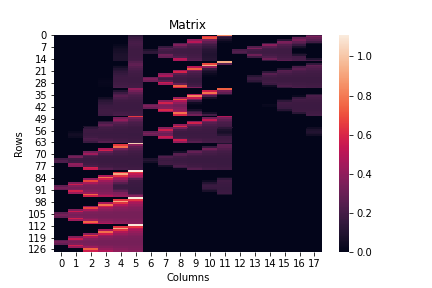
\includegraphics[width=0.7\textwidth]{A_block_1.png}
	\caption{Исходная матрица}
\end{figure}

На следующих графиках представлены сравнения полученных правых частей и исходных и сравнения векторов-решений и истинных решений при выборе 1, 5, 15, 30, 50 или 100 подсистем.
\newpage
\begin{figure}[h]
	\centering
	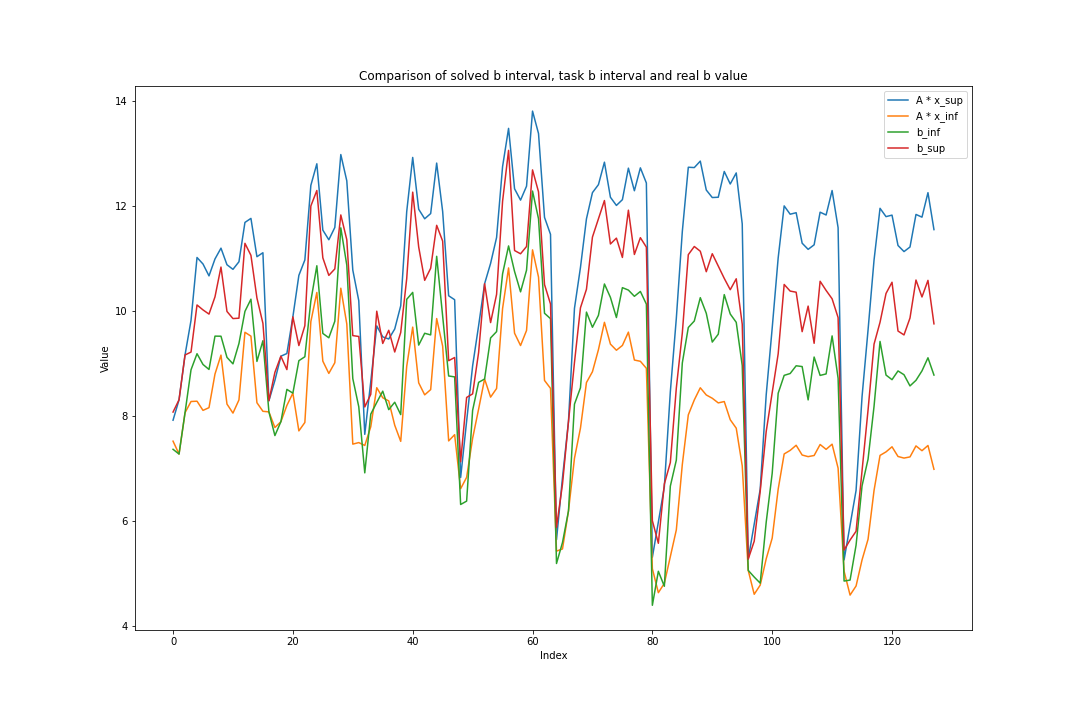
\includegraphics[width=0.7\textwidth]{sols_1_mats_1.png}
	\caption{Сравнение правых частей. 1 подматрица}
\end{figure}

\begin{figure}[h]
	\centering
	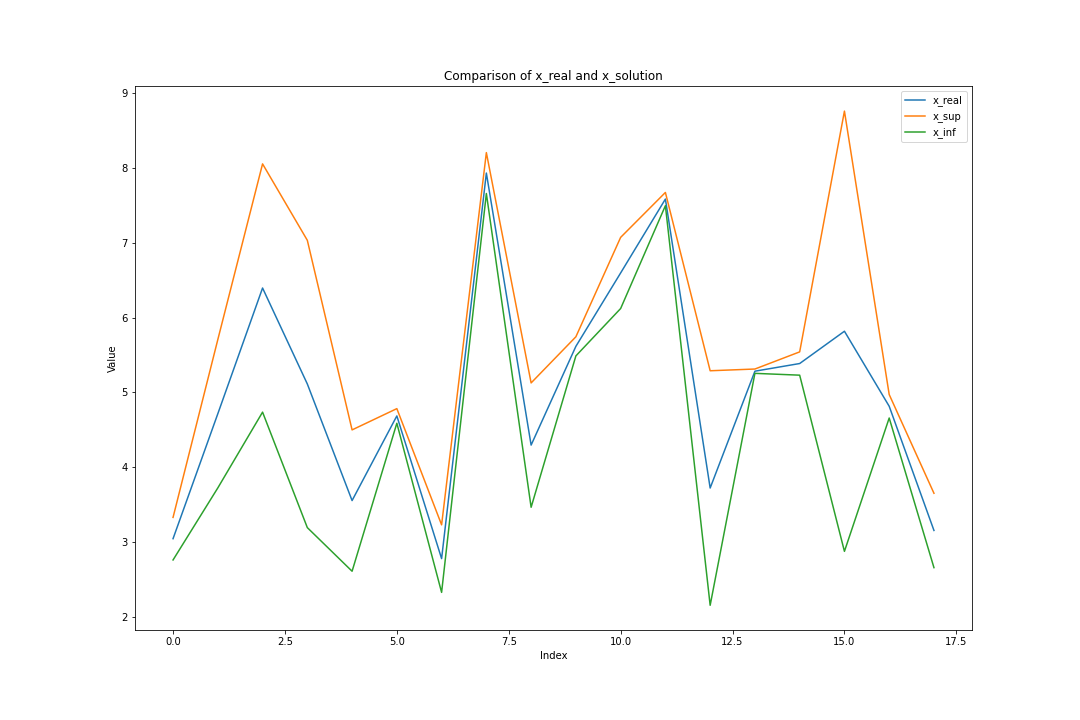
\includegraphics[width=0.7\textwidth]{xs_1_mats_1.png}
	\caption{Сравнение исходного решения и полученного интервального решения. 1 подматрица}
\end{figure}
\newpage
\begin{figure}[h]
	\centering
	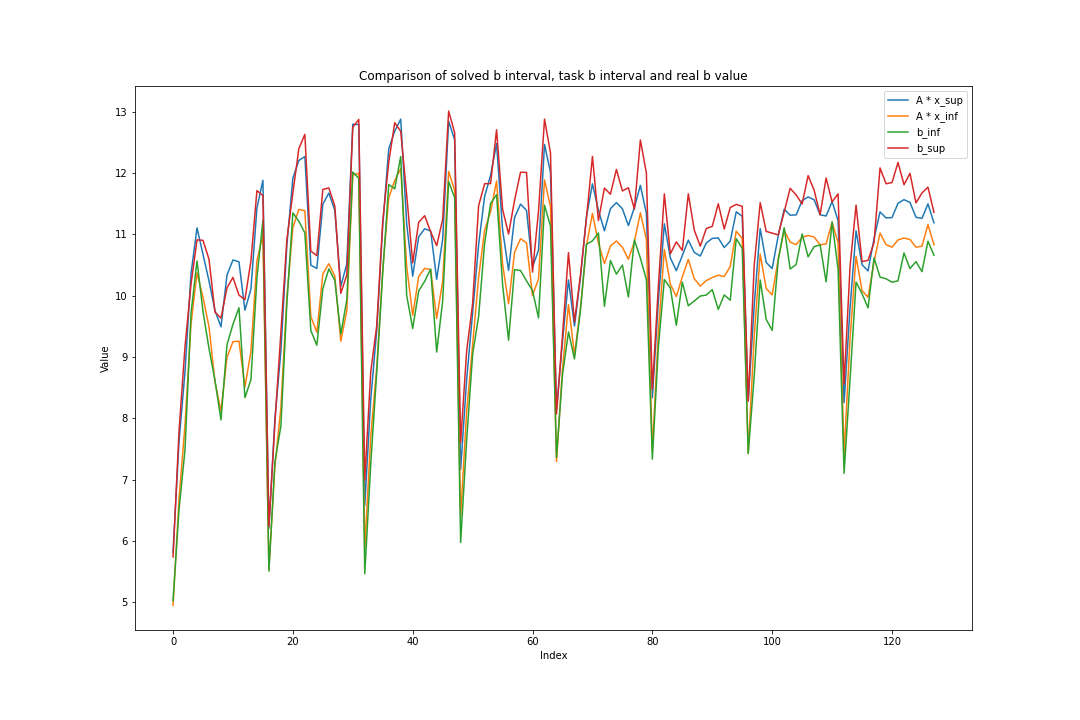
\includegraphics[width=0.7\textwidth]{sols_5_mats_1.png}
	\caption{Сравнение правых частей. 5 подматриц}
\end{figure}

\begin{figure}[h]
	\centering
	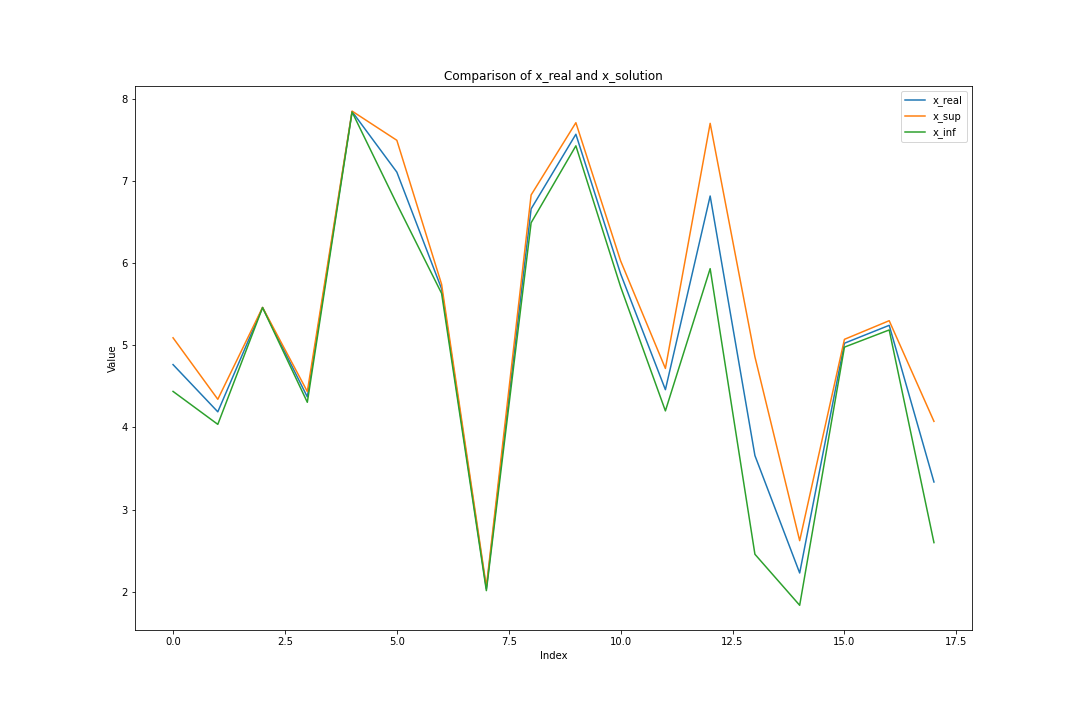
\includegraphics[width=0.7\textwidth]{xs_5_mats_1.png}
	\caption{Сравнение исходного решения и полученного интервального решения. 5 подматрица}
\end{figure}
\newpage
\begin{figure}[h]
	\centering
	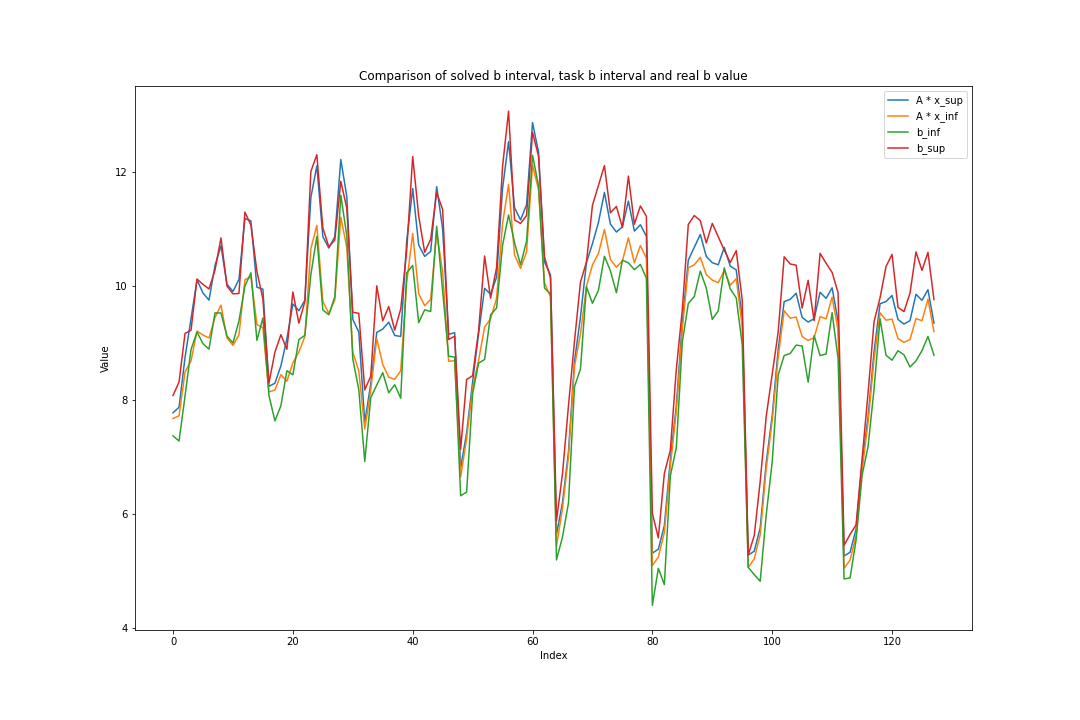
\includegraphics[width=0.7\textwidth]{sols_15_mats_1.png}
	\caption{Сравнение правых частей. 15 подматриц}
\end{figure}

\begin{figure}[h]
	\centering
	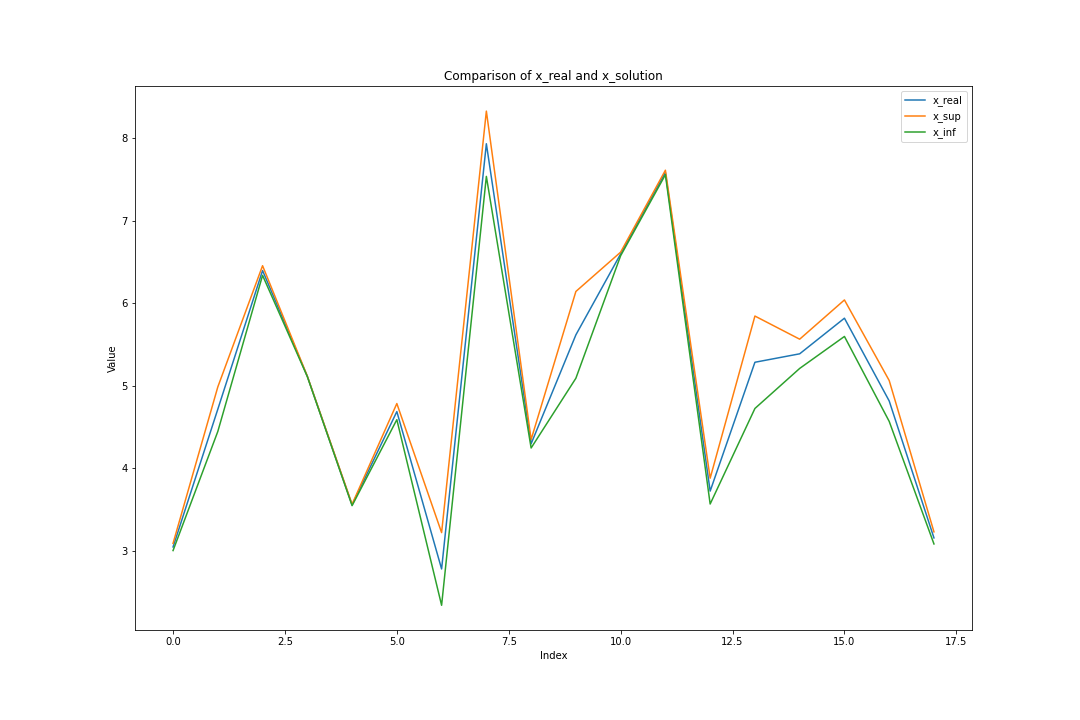
\includegraphics[width=0.7\textwidth]{xs_15_mats_1.png}
	\caption{Сравнение исходного решения и полученного интервального решения. 15 подматриц}
\end{figure}
\newpage
\begin{figure}[h]
	\centering
	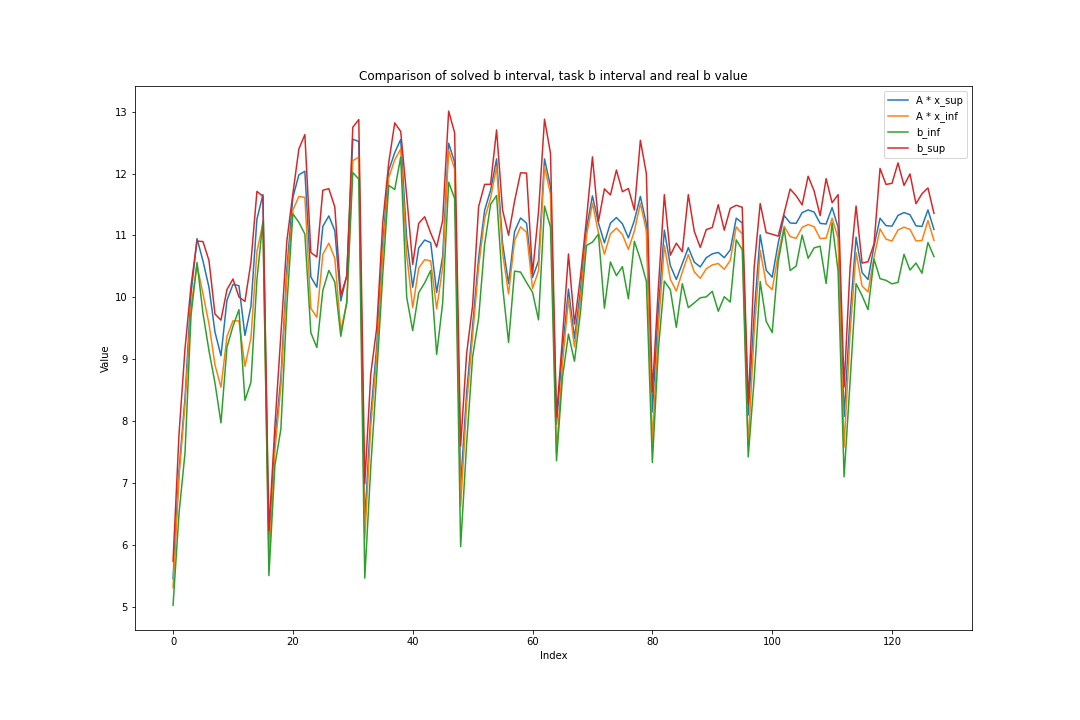
\includegraphics[width=0.7\textwidth]{sols_30_mats_1.png}
	\caption{Сравнение правых частей. 30 подматриц}
\end{figure}

\begin{figure}[h]
	\centering
	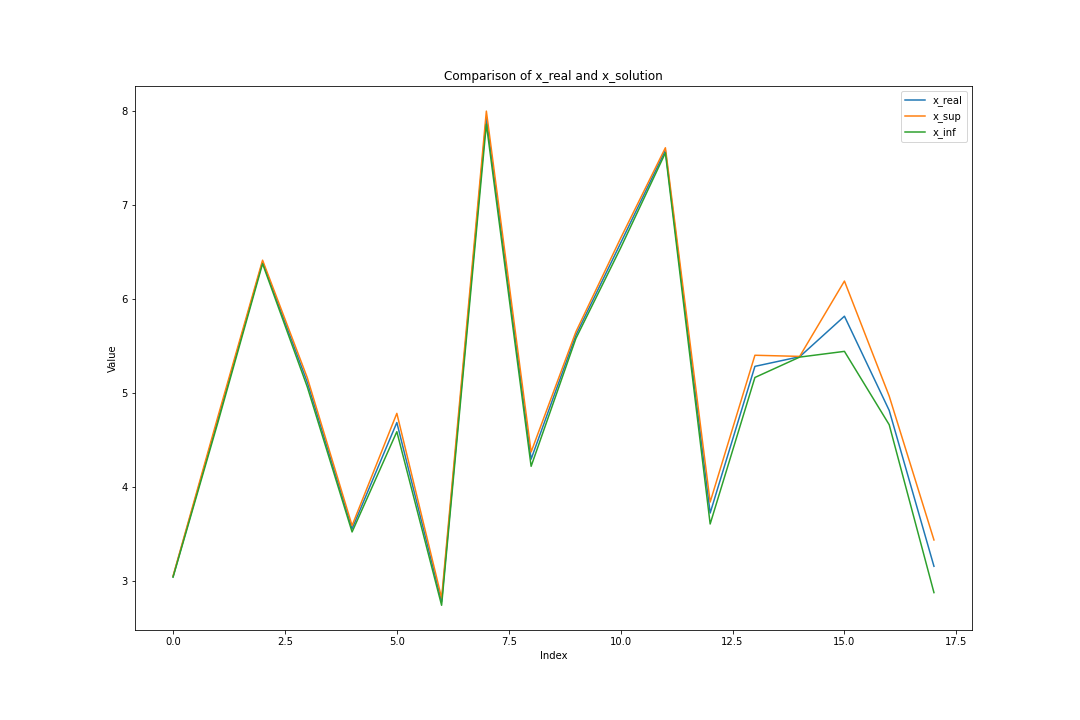
\includegraphics[width=0.7\textwidth]{xs_30_mats_1.png}
	\caption{Сравнение исходного решения и полученного интервального решения. 30 подматриц}
\end{figure}
\newpage
\begin{figure}[h]
	\centering
	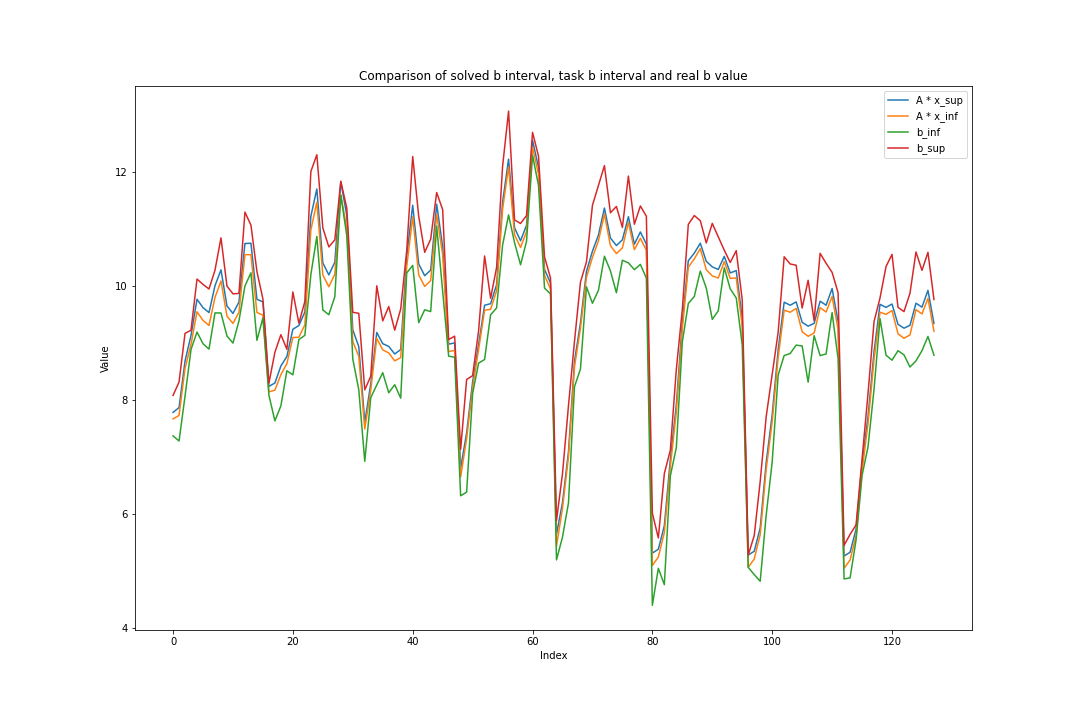
\includegraphics[width=0.7\textwidth]{sols_50_mats_1.png}
	\caption{Сравнение правых частей. 50 подматриц}
\end{figure}

\begin{figure}[h]
	\centering
	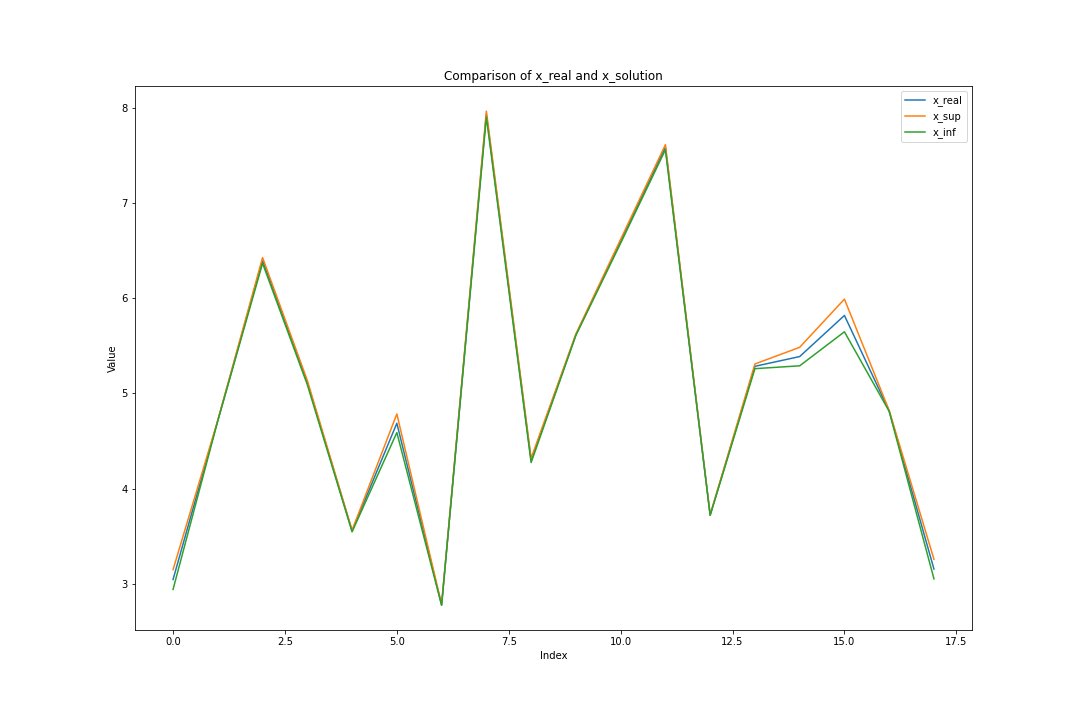
\includegraphics[width=0.7\textwidth]{xs_50_mats_1.png}
	\caption{Сравнение исходного решения и полученного интервального решения. 50 подматриц}
\end{figure}
\newpage
\begin{figure}[h]
	\centering
	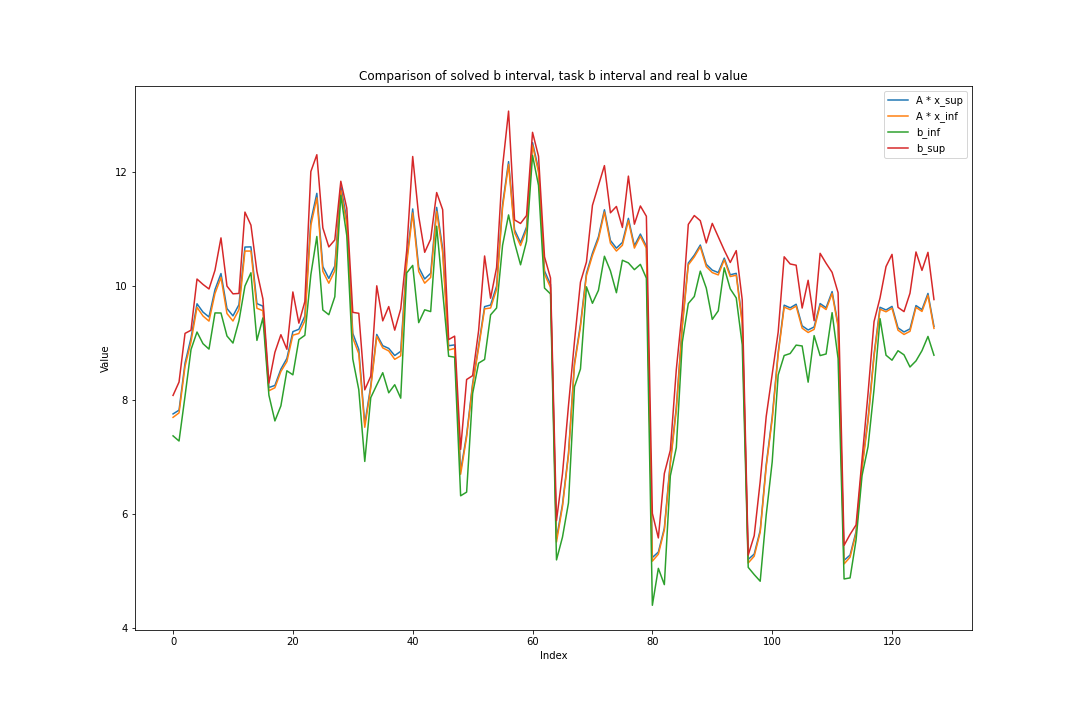
\includegraphics[width=0.7\textwidth]{sols_100_mats_1.png}
	\caption{Сравнение правых частей. 100 подматриц}
\end{figure}

\begin{figure}[h]
	\centering
	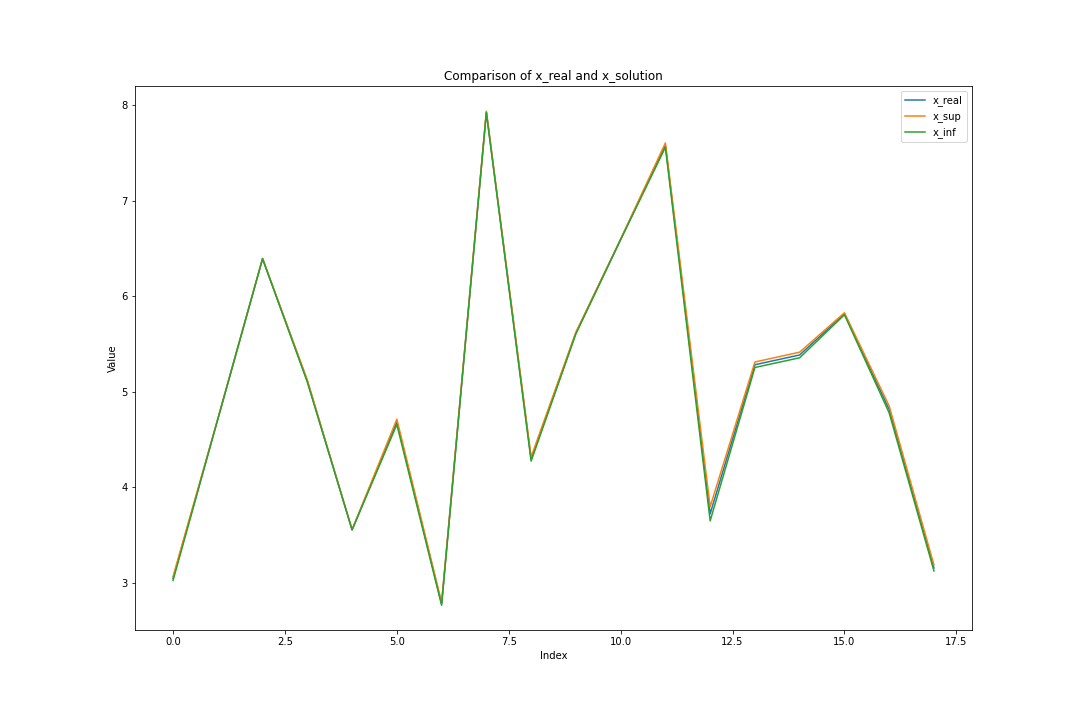
\includegraphics[width=0.7\textwidth]{xs_100_mats_1.png}
	\caption{Сравнение исходного решения и полученного интервального решения. 100 подматриц}
\end{figure}
\newpage


\section{Анализ}
Из графиков видно, что для всех вариантов получаемая правая часть находилась в границах исходной правой части. Более того, при увеличении количества выбираемых подматриц интервалы правой части сужались. \\

Для всех вариантов истинный вектор-решение всегда находился в интервале полученного решения. А при увеличении количества подматриц полученный вектор сужался к истинному. \\

Из этого можно сделать вывод, что при увеличении количества выбираемых матриц решение-пересечение стремится к истинному.



\section{Приложение}
Код программы на Python лежит в данном репозитории: \\
\url{https://github.com/PinkOink/Interval_Analysis/tree/main/course_project}{}


\end{document}